\documentclass[10pt]{article}
\usepackage{graphicx} % Required for inserting images
\usepackage{listings}
\usepackage[a4paper, total={150mm, 237mm}]{geometry}
\usepackage{helvet}
\renewcommand{\familydefault}{\sfdefault}
\usepackage[ngerman]{babel}
\usepackage[T1]{fontenc}
\usepackage{tabularx}
\usepackage{float}
\begingroup\linespread{1.3}
\usepackage{multicol}
\usepackage{minted}
\usemintedstyle{friendly} % Change theme
\usepackage{caption}


\begin{document}

%\renewcommand\thesection{\ifnum\value{section}<5\Roman{section}\else\arabic{section}\fi}
\renewcommand\thesection{\Roman{section}}
\pagenumbering{Roman}
\begin{titlepage}
    \begin{center}
        \begin{multicols}{2}
            
\includegraphics[scale=.3]{dateien/THI_Logo.jpg} \\
            \vspace{0.5cm}
            Technische Hochschule Ingolstadt\\
            \columnbreak
            
\includegraphics[scale=.2]{dateien/EXP Logo.png} \\
            \vspace{1.5cm}
            EXP Software GmbH\\
        \end{multicols}
        \vspace{1cm}
        \normalsize
        Andreas Dinauer\\
        and2925@thi.de\\
        
        \vspace*{0.5cm}
        \LARGE
        \textbf{Konzeption und Entwicklung eines Systems zum Aufbau eines Wissensgraphen aus einem Jira-System}
            
        \vspace{1cm}
        \normalsize
        Erstprüfer/-in: Prof. Dr. Hans-Michael Windisch \\
        Zweitprüfer/-in: Prof. Dr. Beate Navarro Bullock \\
        \vspace{1cm}
        \normalsize
        Externer Partner: EXP Software GmbH
            
    \end{center}
\end{titlepage}

\newpage

\section{Inhaltsverzeichnis}

\renewcommand{\contentsname}{}
\tableofcontents
\newpage
\section{Abkürzungsverzeichnis}
\newpage
\section{Abbildungsverzeichnis}
\renewcommand{\listfigurename}{}
\listoffigures
\newpage
\section{Tabellenverzeichnis}
\renewcommand{\listtablename}{}
\listoftables{}
\newpage
\setcounter{section}{0}
\renewcommand\thesection{\arabic{section}}
\pagenumbering{arabic}
\section{Einleitung in das Wissensmanagement durch KI}
\subsection{Einleitung}
Heutzutage ist die Analyse von Daten in vielen Unternehmen wichtiger als je zuvor und die Gewinnung von Wissen aus Daten gewinnt stetig an Stellenwert. Passend zu dieser Beobachtung schreibt das Marktforschungs- und Beratungsunternehmen Gartner: "Graph analysis is possibly the single most effective competitive differentiator for organizations pursuing data-driven operations and decisions". (Gartner, 2014, zitiert in Robinson, 2015, S. 2) \\
Durch die Einführung einer Künstlichen Intelligenz, um das Wissensmanagement im Unternehmen zu verbessern ergeben sich mehrere Teilaspekte im Umgang mit Wissen. Neben der Möglichkeit, durch das Transformieren von bereits vorhandenem Wissen, um neues Wissen zu kreieren, kann eine Künstliche Intelligenz auch den Prozess des Abfragens und Extrahierens von Wissen aus einer großen Sammlung an Daten unterstützen. Diese Arbeit beschäftigt sich primär mit dem Aspekt der Wissensabfrage und dem Aufbau der hierfür notwendigen Datenstrukturen. (vgl. Jarrahi, 2023, S. 2) \\
Durch die Entwicklung und Bedeutung von Wissensgraphen in der heutigen Zeit sowie die revolutionären Entwicklungen im Bereich der künstlichen Intelligenz ergeben sich für Unternehmen neue Möglichkeiten, das Wissensmanagement in ihrem Betrieb neu zu gestalten. Ziel dieser Arbeit ist es, ein System zu entwerfen und zu implementieren, welches die Erstellen eines Wissensgraphen ermöglicht, der speziell für die Integration mit einem Chatbot, insbesondere einem Large Language Model (LLM), konzipiert ist.\\
Um Chatbots im Unternehmenskontext einsetzen zu können, müssen diese mit dem Unternehmensumfeld, also den Daten und Abläufen des Unternehmens vertraut gemacht werden. Dazu wird untersucht, wie ein Knowledge Graph aus einer bereits existierenden und stetig weiter wachsenden Sammlung aus Tickets eines Jira-Systems erstellt werden kann. Berücksichtigt werden hierbei Duplikate, Dateninkonsistenzen, sowie die Historisierung und Auditierung. Der Hauptaspekt dieser Arbeit ist das Design, sowie die Implementierung des Datenbankschemas und der Extraktor-Komponente. Am Ende wird geprüft, ob sich eine Graphdatenbank für die Integration eines Chatbots eigenet, um möglichst schnell und präsize das Informationsbefürdnis eines Anwender zu befriedigen.\\
Außerdem werden zusätzlich zu den Herausforderungen beim Aufbau des Graphen, mögliche Herausforderungen in Verbindung mit der Data Warehouse Architektur behandelt. Teil dessen sind beispielsweise die Terminierung der Extraktion, das Speichern der Metadaten sowie die Konfiguration des Extraktors, der das extrahieren der Jira Daten vornimmt. \\
\subsection{Vorgehensweise}
Die Struktur dieser Arbeit folgt dem Ansatz des Wasserfallmodells in der Softwareentwicklung. Zu Beginn erfolgt die Anforderungsanalyse. Dabei soll festgelegt werden, welche funktionlen und nicht-funktionalen Anforderungen unser System erfüllen muss und welche optional erfüllt werden sollen. In Folge des Anforderungsmanagements müssen alle Bestandteile des Systems, wie z. B. Datenbankmodelle, Datenbanken sowie Softwarekomponenten mit Applikationslogik identifiziert werden, welche notwendig sind, um den Prozess zum Erstellen des Knowledge Graphen durchzuführen. Anschließen soll dargelegt und begründet werden, für welche konkreten Ausführungen, Implementierungen und Technologien entschieden wird. Es sollen alle signifikanten Vor- und Nachteile erläutert werden. Es soll beschrieben, warum sich diese Technologien gut für eine Integration eignen. Sobald alle Bestandteile des Systems festgelegt sind, wird mit der Planung, dem Design und der Implementierung des Systems begonnen. In dieser Phase werden alle Jira-Objekte erfasst und als Datenbankschema modelliert. Es folgt eine genaue Beschreibung, wie beispielsweise ein Datenbankschema modelliert wird. Außerdem wird beschrieben, wie die ermittelten Anforderungen in Form von Code umgesetzt werden. Bei der Implementierung des Codes sollen zentrale Aspekte und Abschnitte im Code aufgegriffen und genauer erläutert werden. Anschließend wird die Integration sowie die Einführung der Software erläutert. Zuletzt soll geprüft werden, wie eine Künstliche Intelligenz möglichst effizient mit diesem Knowledge Graphen als Datengrundlage integriert werden kann.\\
\section{Konzeption und Planung des Systems}
\subsection{Aufbau des Systems}
\subsubsection{Architektur}
Das System besteht aus drei verschiedenen Komponenten, dem Quellsystem, einem Extraktor sowie einem Zielsystem. Im Quellsystem befinden sich die Rohdaten aus dem operativen Betrieb. Diese sollen mit Hilfe des Extraktors extrahiert und im Zielsystem strukturiert abgespeichert werden. Während es sich beim Quellsystem um eine Jira Cloud-Instanz handelt, ist das Zielsystem eine NoSQL-Datenbank. Der Extraktor ist ein Softwareprogramm, welches periodisch zur Ausführung gebracht wird.
\subsubsection{Konzept des Data Warehouses}
Die Architektur unseres Systems ist einem Data Warehouse sehr ähnlich und erfüllt alle Eigenschaften eines Data Warehouses nach Inmon. Diese Erkenntnis unterstützt beim Entwurf des Systems und ermöglich es, Konzepte, Best Practices und Technologien im Zusammenhang mit dem Data Warehouses einzusetzen.
\begin{itemize}
  \item Historisierung: Alle Objekte des Jira Systems sind mit einem Zeitstempel der letzten Änderung, sowie der Erstellung versehen, was den Aufbau eines historisierten Datenbestandes ermöglicht.
  \item Integriert: Wir extrahieren unsere Daten aus nur einem System. Das Hinzufügen eines weiteren Jira-Systems ist möglich und wird in der Architektur des Systems berücksichtigt.
  \item Nicht-Volatilität: Der Datenbestand wird dauerhaft aufgebaut und bleibt bestehen. In Gegensatz zu operativen Systemen werden aus unserem Zielsystem keine Daten gelöscht.
  \item Fach-orientiert: Unser Datenbestand hält fachliche Daten aus dem operativen Geschäftsablauf.
\end{itemize}
[ZITAT]\\\\
Der Aufbau des Systems und dessen Komponenten sind angelehnt an bereits existierende Referenzmodelle für Data Warehouses. Der Datenbestand des Data Warehouse soll mit hilfe eines ETL-Prozesses aufgebaut werden. Dabei werden Daten aus einem Jira-System (Quellsystem) extrahiert, transformiert und dann in die Graphdatenbank (ArcadeDB) geladen. Außerdem gibt es ein Metadaten-Repository, um Daten über den Extraktionsprozess und dessen Daten zu speichern. Dieses Metadaten-Repository wird unter anderem dazu dienen die genauen Ausführungszeiten, sowie die Token der Texte. Abbildung 1 gibt einen vereinfachten Überblick über das System und dessen Komponenten.
\begin{figure}[h]
\centering
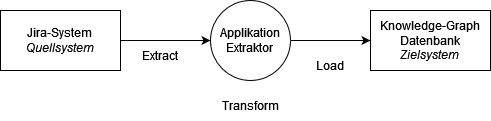
\includegraphics[scale=.6]{dateien/ETL-Prozess.jpg}
\caption{Der ETL-Prozess zum Aufbau des Knowledge Graphen}
\label{fig:meine-grafik}
\end{figure}
\subsection{Anforderungserhebung}
Um die gesamte Applikation und und dessen Komponenten besser zu verstehen und bessere Anforderungen formulieren zu können, betrachten wir dieses als System. Die einzelnen Bestandteile wiederum können jeweils als Subsystem bezeichnet werden. Ist unser System mit einem externen System integriert, so wird dieses als Umsystem bezeichnet. In unserer Architektur entspricht das Jira-System einem Umsystem. Als Subsystem werden alle Beständeteile betrachtet, welche dem System vollständig angehören. Die Graph-Datenbank, der Jira-Extraktor und eine Datenbank zur Speicherung von Konfigurations- sowie Metadaten wären somit Subsysteme. [978-3-658-37194-4, S.60] \\
Zunächst müssen die Anforderungen an das System erhoben und kategorisiert werden. Dabei wird zwischen funktionalen und nicht-funktionalen Anforderungen unterschieden. Alle in diesem Kapitel erhobenen Anforderungen sind so gestaltet, dass die Applikation im beliebigem Kontext  und dynamisch eingesetzt werden kann. Den Anforderungen liegt kein spezifischer Anwendungsfall zugrunde.\\
Es gibt vier verschiedene Ansätze zur Erfassung für Anforderungen. Die folgenden Anforderungen wurden alle auf Basis eigener Überlegungen und ersten Code-Ausführungen durch den Ansatz "Kreativität" erhoben. Für eine Beobachtung oder das Untersuchen von Artifakten sind keine Ressourcen wie z.B. Dokumente oder bereits bestehende Anforderungen verfügbar.[978-3-658-37194-4, S.60]. \\
Jeder Stichpunkt beschreibt eine Anforderung an das System, einer Komponente des Systems oder einen Ablauf im System und wird nach einem bestimmten Schema formuliert. Einer Anforderung kann eine bestimmte Verbindlichkeit zugeordnet werden, welche durch die Formulierung der Anforderung deutlich wird. Muss eine Anforderung umgesetzt werden, so hat diese die höchste Priorität und ist für die grundlegende Fertigstellung der Applikation unerlässlich. Soll eine Anforderung umgesetzt werden, so schafft diese einen deutlichen Mehrwert und verbessert die Applikation signifikant. Kann eine Anforderung umgesetzt werden, so handelt es sich dabei um eine optionale Erweiterung, welche nur umgesetzt wird, wenn die notwendigen Resourcen verfügbar sind.\\
Im Anschluss an die Anforderungserhebung werden die Randbedingungen durch einen Vergleich von verschiedenen Technologien festgelegt.
\subsubsection{Funktionale Anforderungen}
Funktionale Anforderungen beschreiben die fachliche Spezifikation eines Systems, sowie alle Schnittstellen inklusive der Eingangs- sowie Ausgabeparameter des Systems. Diese Anforderungen werden in der Testphase der Entwicklung in Testfälle überführt. Können die Tests erfolgreich ausgeführt werden, so erfüllt die Applikation die zuvor festgelegten Anforderungen.\\
Folgende funktionale Anforderungen müssen erfüllt sein:
\begin{itemize}
  \item Das System muss genau eine Jira-Cloud Instanz als Datenquelle verwenden. 
  \item Die Interaktion mit der Jira-Cloud API in Java soll mittels der breits von Atlassian bereitgestellten Dependencies umgesetzt werden. Es soll Basic-Authorization verwendet werden. Als Java Build-Tool soll Maven verwendet werden.
  \item Es soll möglich sein, diese Projekte genau zu konfigurieren. Dabei soll es auch möglich sein, für jedes Projekt die zu extrahierenden Vorgangstypen festzulegen. Der Speicherort zu dieser Konfigurationsdatei muss durch Umgebungsvariablen dynamisch konfigurierbar sein. Folgende JSON-Datei gibt unserer Applikation die Anweisung, den Issuetype Task und Bug des Projektes mit dem Schlüssel KAW und den Issuetype Story und Task des Projektes mit dem Schlüssel MUN zu extrahieren und in das Zielsystem zu laden:
    \begin{minted}{json}
    {
        "KAW": ["Task", "Bug"],
        "MUN": ["Story", "Task"]
    }
    \end{minted}
  \item Das System muss dynamisch durch das Konfigurieren der Datenbankverbindung mittels Umgebungsvariablen an die Zieldatenbank angebunden werden. Dabei muss der Name und das Passwort des Benutzers, sowie der Host, der Port und das Schema der Datenbank konfiguriert werden können.
  \item Das System soll beim extrahieren eines Jira Tickets und eines Jira Subtasks erkennen, ob ein Duplikat vorliegt und beim einfügen in die Zieldatenbank eine Verknüpfung herstellen, welche eine Aussage trifft, wie ähnlich beide Objekte sind.\\
  Um die Duplikatprüfung durchzuführen soll das System auf die Schlüsselwörter zurückgreifen, welche sich in den relevanten Werten von Attributen eines Objektes befinden. Teil dieser Attribute sind beispielsweise der Titel oder die Beschreibung eines Tickets.
  \item Die Applikation muss den ETL-Prozess beim Start der Anwendung durchführen und nach Beendigung des ETL-Prozess mit einem Fehlercode terminieren.
  \item Das System soll nicht eigenständig die zeitliche Ausführung terminieren sondern von seiner Umgebung zur Ausführung gebracht werden. Beispielsweise kann die Terminierung in einem Kubernetes Cluster stattfinden. Ein Vorteil wäre, dass in diesem Fall mehrere Knoten zur Verfügung stehen, welche eine höhere Ausfallsicherheit garantieren. Des weiteren haben sich externe Scheduling-Methoden im Gegensatz zur selbständigen Implementierung als sehr zuverlässig erwiesen. \\
  \item Das System soll alle neuen oder geänderten Objekte periodisch exportieren. Ein Exportvorgang soll einmal pro Tag stattfinden. Ein Exportvorgang soll immer zur gleichen Tageszeit und außerhalb der Zeit geschehen, in welcher mit dem Zielsystem gearbeitet wird.
  \item Das System soll alle relevanten Objekte exportieren, die ein Jira-Projekt umfassend beschreiben. Diese sind z.B. Vorgänge, Vorgangstypen, Projekte und Kommentare.
  \item Das System muss alle Daten auf die Zieldatenbank transformieren. Alle für die Analyse nicht relevanten Metadaten aus dem Jira-System sollen aussortiert werden. Ausschließlich wichtige Felder für die folgende Analysen sollen in ein angemessenes Format transormiert werden.
  \item Die Extraktion eines jeden Objektes soll dokumentiert werden. Hierzu werden alle Vorgänge in einer Datenbank erfasst. Zu jedem Vorgang werden mindestens der Zeitpunkt, der Typ und die Kennung eines Objektes erfasst.\\
  Falls bei einem Teilvorgang der Extraktion ein Fehler auftritt und das zugehörige Objekt nicht extrahiert und geladen werden kann soll ein Log-Eintrag bezüglich des Objekts in strukturierter und maschinenlesbarer Sprache erzeugt werden. Dies ermöglicht in Zukunft eine weitere Fehlerbehandlung.
  \item Die Applikation muss Änderungen an Objekten erkennen und diese historisieren, also alle Änderungen in einen zeitlichen Zusammenhang bringen und ordnen können.
\end{itemize}

Folgende funktionale Anforderungen sollen erfüllt sein:
\begin{itemize}
  \item Die Zieldatenbank soll für effiziente Analysen geeignet sein und Objekte effizient miteinander verknüpfen. Dadurch sollen möglichst schnell Verknüpfungen sowie ein Kontext hergestellt werden können.
  \item Die Zieldatenbank soll für sehr große Datenmengen konzipiert sein, da alle Objekte versioniert werden und somit mehrfach speichern werden.
\end{itemize}
Folgende funktionale Anforderungen können erfüllt sein
\begin{itemize}
  \item Der Extraktor kennt für jeden Extraktionsvorgang sowie den Gesamtvorgang die benötigte Zeit und speichert diese für spätere Analysen.
\end{itemize}
\subsubsection{Nicht-funktionale Anforderungen}
Nicht-funktionale Anforderungen beschreiben den Aufbau des Systems. Auch sie werden in Form von Testfällen nach Beenden der Entwicklung geprüft und müssen für eine erfolgreiche Entwicklung erfüllt sein.\\
Folgende nicht-funktionale Anforderungen müssen erfüllt sein:
\begin{itemize}
\item Das System muss alle Extraktionsvorgänge in einer Datenbank dokumentieren und falls eine Ausführung nicht stattgefunden hat, dieses erkennen, diese bis zu einem gewissen Zeitpunkt nachholen. Eine Ausführung kann beispielsweise nicht stattfinden, wenn das System zum geplanten Zeitpunkt nicht lauffähig ist. Wird die Applikation später gestartet, soll diese mit der Ausführung beginnen.
\item Das Systen muss weitestgehend fehlerfrei arbeiten. Insbesondere müssen alle vorgesehenen Objekte extrahiert werden. Es darf kein Objekt, welches geändert oder neu erstellt wurde ohne Export im Quellsystem (durch z.B Fehler mit dem Zeitstempel durch Latenzen bei der Anfrage) verbleiben.
\item Das System muss eine hohe Fehlertoleranz aufweisen und verschiedene Mechanismen implementieren, welche eine hohe Resilienz des Systems gewährleisten. Falls in einem Extraktionsvorgang eine Ausnahme auftritt, so muss durch einen Logeintrag erkennbar sein, bei welchem Objekt und Objekttyp oder Jira-Schnittstelle diese verursacht wurde. Ein weiterer Versuch, das entsprechende Objekt zu extrahieren, soll beim nächsten regulären Extraktionsvorgang angestoßen werden.
\item Das System muss flexibel gestaltet sein und alle notwendigen Parameter zur Extraktion durch Umgebungsvariablen erhalten. Wichtige Parameter sind beispielsweise der Jira Benutzer, dessen Passwort und die URL der Jira Instanz. Ein Pfad zur Konfigurationsdatei aller relevanten Jira-Projekte sowie Vorgangstypen, welche zur Extraktion bestimmt sind, soll auch durch eine Umgebungsvariable gesetzt werden können.
\item Die Applikation muss speziell für containerisierte Umgebungen und Cloudumgebungen bestimmt sein und somit als Image für IaC-Anwendungen (z.B. Docker oder Kubernetes) ausführbar sein.
\end{itemize}
Folgende nicht-funktionale Anforderungen sollen erfüllt sein:
\begin{itemize}
  \item Der Extraktor soll nicht skalierbar sein. Es ist nur eine Instanz für jeweils einen Extraktionsvorgang vorgesehen. Ein Entwurf, um das System als Cluster zu betreiben ist sinnvoll, wird aber aufgrund von übermäßigem Aufwand bei der Implementierung der Kommunikation zwischen Instanzen nicht umgesetzt. Die Zieldatenbank muss aber in der produktiven Umgebung als verteilte Datenbank kompatibel mit dem Extraktor sein.
  \item Die Applikation soll möglichst intuitiv konfiguriert werden können und durch möglichst wenig Umgebungsvariablen konfiguriert werden können.
\end{itemize}
Es werden keine Anforderungen an die Extraktionsdauer gestellt. Dies ergibt sich daraus, dass die Applikation als Hintergrundprozess ausgeführt wird und durch einen langen ETL-Prozess kein Anwender beeinträchtigt wird. Primäres Ziel der Applikation ist die Extraktion und Aufbereitung von fachlich korrekten und konsistenten Daten. Außerdem ist vorgesehen, die Anwendung gezielt auszuführen, wenn möglichst keine Anwender mit dem System interagieren. Ressourcen zur Optimierung der Ausführungsdauer werden daher gezielt eingesetzt, um die Fehlerfreiheit der Applikation zu verbessern.

\section{Auswahl der Softwarekomponenten}
Im folgenden wird begründet, warum eine bestimmte Technologie ausgewählt wird und wie diese unser System ergänzt und warum diese optimal mit anderen Komponenten integriert werden kann.
\subsection{Auswahl eines geeigneten Extraktors}
Der Extraktor unseres Systems implementiert den ETL-Prozess und bringt diesen zur Ausführung. Seine Aufgabe ist das extrahieren der Daten, das transformieren der Daten in das Format des Zielsystems sowie das Laden der Daten in das Zielsystem. Implementiert wird dieser in der Programmiersprache Java. Grund hierfür ist, dass Java sehr weit verbreitet und etabliert ist sowie eine große Auswahl Frameworks und Bibliotheken bei der Entwicklung bietet. Zur Unterstützung in der Entwicklung wird ein Framework verwendet. Aus verschiedenen Gründe wird Quarkus eingesetzt. Ein großer Vorteil des Frameworks ist, dass es unter der Apache License 2.0 als Open Source Software eingesetzt werden kann. Außerdem bietet Quarkus eine sehr umfangreiche Auswahl an Erweiterungen für verschiedene Anwendungsfälle und unterstützt durch eine große Auswahl an Funktionen auch die Integration mit anderen Softwarekomponenten und Technologien. In der Praxis werden Anwendung in der Cloud häufig nach Rechenzeit und Speicherbedarf abgerechnet. Somit gewinnt die Optimierung der Anwendung auf Speicher- und Rechenzeitbedarf immer mehr an Wichtigkeit. Quarkus zeichnet sich durch eine schnelle Startzeit sowie die Optimierung für Container-Technologien und somit für Cloud-Umgebungen aus.\\
Ein weiterer Vorteil der Quarkus-Frameworks ist die Implementierung der Jakarta WS RS Schnittstelle, welche grundlegende Funktionalitäten für eine Unternehmensanwedung bietet. Die Implementierung einer offenen Spezifikation ermöglicht einen nahtlosen Umstieg auf ein alternatives Framework, welches ebenfalls diese Spezifikation implementiert, falls dieses notwendig ist. Alternative Frameworks wie z.B. Spring Boot implementiert z. T. proprietäre Spezifikationen und erschwert somit einen Wechsel, da häufig eine erneute Implementierung notwendig ist. Des weiteren bietet Quarkus Funktionen, um die Produktivität während des Entwickelns start zu verbessern. Eine Eigenschaft des Frameworks ist der Hot-Reload, welcher alle Änderungen des Codes automatisch in die laufende Entwicklungsinstanz einbringt und keinen Neustart der Anwendung erfordert. (vgl. Koleoso, 2020, S. 8)
\subsection{Auswahl eines geeigneten Datenbankmodells}
Der Mehrwert der Applikation für einen Anwender entsteht durch die Auswertung der Daten in unserem Zielsystem. Daher ist es besonders wichtig, auf ein Datenbankmodell zurückzugreifen, welches unseren Anwendungszweck, also das Integrieren mit einem Chatbot bestmöglich unterstützt. Im folgenden werden Datenbanken welche bei sehr spezifische Anwendungszwecken zum Einsatz kommen wie z.B eine Zeitstempel-Datenbank oder eine Key-Value-Datenbank nicht weiter betrachtet. Zur Auswahl stehen eine relationale Datenbank oder eine Graph-Datenbank. Um eine Entscheidung zu treffen, werden die beiden Datenbankmodelle anhand verschiedener Kriterien in Bezug zu unserem Anwendungsfall bewertet. Jedes Kriterium besitzt dabei eine Gewichtung. Ist das Kriterium besonders ausschlaggebend so ist die Gewichtung hoch. Eine ausführliche Erörterung der Kriterien folgt im Anschluss an die Tabelle.
\begin{table}[H]
\caption{Das Relationale und das Graph-Datenbankmodell im Vergleich}
    \begin{tabularx}{\textwidth}{|X|X|X|X|}
    \hline
    \textbf{Kriterium} & \textbf{Gewichtung} & \textbf{Relationale Datenbanken} & \textbf{Graph Datenbanken} \\ \hline
    Verknüpfungen         & 0,5         & 0 &  0 \\ \hline
    Skalierbarkeit         & 0,3         & Eintrag 6   & Eintrag 3        \\ \hline
    ACID-Eigenschaften         & 0,2         & 1,0    & 0,2      \\ \hline
    \textbf{Ergebnis}         &    0     & \textbf{1,0}    & \textbf{0,2}      \\ \hline
    \end{tabularx}
\end{table}
Verknüpfungen sind in unserem Anwendungsfall essenziell und werden somit stark gewichtet. Relationale Dantenbanken verbinden Entitäten durch logische Verknüpfungen. Während dieses Vorgehen für eine gute Lesbarkeit für menschliche Anwender bietet, wird dadurch die Zeit einer Anfrage beeinträchtigt. Folgende Grafik vergleicht die Abfragezeiten vom Finden von Entitäten, welche durch eine bestimmte Tiefe (Anzahl der Verknüpfungen) von der Ausgangsentität entfernt sind.

\begin{figure}[H]
\centering
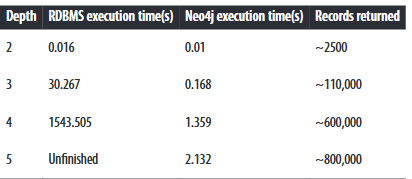
\includegraphics[scale=.6]{dateien/table.png}
\captionsetup{font=small, labelfont=bf, justification=centering}
\caption{Vergleich der Abfragezeit von Entitäten in RDBMS und Graph Datenbanken (vgl. Robinson, Webber und Eifrem, 2025, S. 21)}
\label{fig:meine-grafik}
\end{figure}
Graph Datenbanken implementieren die Verknüpfungen von Entitäten durch physische Pointer. Es wird eine Relationale Datenbank mit einer Graph Datenbank verglichen (Neo4J). Hierbei wird direkt der Speicherort referenziert. Für unseren Einsatzzweck benötigen wir eine Datenbank, welche stark auf die Verknüpfung von Daten optimiert ist und bewerten somit die Graph Datenbank höher.\\
Graph Datenbanken erreichen eine höhere Skalierbarkeit im Vergleich zu relationalen Datenbanken. Dies wird in Abbildung 2 ebenfalls sichtbar. Es zeigt sich ein sehr starker Anstieg der Ausführungszeit bei Relationalen Datenbankmanagementsystemen und ein weniger starker Anstieg bei Graph Datenbankmanagementsystemen. Dies deutet darauf hin, dass Graphdatenbanken effizienter mit großen Datenmengen umgehen können.
\subsection{Chancen und Eigenschaften von Graphdatenbanken}
Graphdatenbanken bestehen aus Knoten und Kanten. Knoten werden mittels Kanten miteinander verbunden und ermöglichen somit ein traversieren der Datenstruktur. Des Weiteren besteht die Möglichkeit den Kanten mit Werten zu versehen, welche als Gewichtung oder Distanz dienen können und somit die Verknpüfung zwischen zwei Knoten quanitifizieren und genauer beschreiben. Graphen, welche Kanten beinhalten, die mehr als 2 Knoten miteinander verknüpfen werden Hypergraphen genannt. Kanten die mehr als 2 Knoten verknüpfen werden Hyperkanten genannt [ZITAT Limitations of graph Databases]. \\Auch wenn eine Graphdatenbank andere Eigenschaften als eine Relationale Datenbank aufweist, finden sich dennoch Elemente aus einer Relationalen Datenbank wieder. Beispielsweise werden Knoten und Kanten als Tabellen gespeichert. Alle Knoten eines Types können mitsamt dessen Attribute wie bei einer relationalen Datenbank per Abfrage ausgegeben werden.\\
Durch den Einsatz von Kanten können Knoten sehr einfach miteinander verknüpft werden. Im Gegensatz zu Relationalen Datenbanken sind somit keine Joins mehr notwendig, da Knoten auf ebene der Datenhaltung direkt miteinander verknüpft werden. Dadurch werden Strukturen geschaffen, welche von einer Künstlichen Intelligenz relativ einfach verknüpft und zu einem Sachverhalt zusammengeführt werden können.
Graphdatenbanken können extrem schnell durchsucht werden und es können Muster im Aufbau des Graphen entdeckt werden.\\
% Leistung und Skalierbarkeit von Graphdatenbanken
Graphdatenbanken sind gut geeignet für große Datenmengen. Graphdatenbanken, die im Bereich Big Data eingesetzt werden, werden als \glqq Big Graphs\grqq\: bezeichnet und können bis zu 1 Milliarde Knoten enthalten, welche durch bis zu 140 Milliarden Kanten miteinander verknüpft sind.\\
% Wo werden diese Datenbanken eingesetzt
Graph Datenbanken decken ein großes Einsatzgebiet ab und werden meist dann eingesetzt, wenn die zu Grunde liegenden Daten stark verknüpft sind. Dies ist u. A. bei sozialen Netzwerken, Wissensgraphen und bei sogenannten Recommendation Engines, also Systeme, welche Vorschläge basierend auf existierenden Daten liefern, der Fall. So können Graphdatenbanken sehr gut mit Verknüpfungen umgehen. Ein weiterer Anwendungsfall für welchen sich Graphdatenbanken gut eignen sind im Umgang mit Daten, welche nur eine schwache Struktur aufweisen. [ZITAT Limits of Graph Databases] \\
Die Entwicklung und Leistung der aktuell verfügbaren Graphdatenbanken gilt als ein entscheidender Faktor für die Entwicklung von leistungsstarken Künstlichen Intelligenzen. (vgl. Fensel et al. 2020, S. 96)
\subsection{Überblick über die Jira Cloud}
Dieses Kapitel gibt einen Überblick über die wichtigsten Aspekte und Elemente in Jira und wozu diese verwendet werden. Die Jira Software ermöglicht das Verwalten von Arbeitsvorgängen, welche als Tickets im System angelegt werden können. Jira-Tickets können in verschiedenen Arbeitsbereichen wie z.B dem Projektmanagement oder der Softwareentwicklung eingesetzt werden, um Aufgaben zu planen. Die Jira Software steht als hybrides Modell zur Verfügung und kann demnach als Data-Center Version selbstständig betrieben oder als Cloud Produkt gebucht werden. Die Inhalte dieser Arbeit basieren auf der Cloud Version der Jira Software. Das System unterstützt primär die Durchführung von Projekten durch den Einsatz von agilen Vorgehensmodellen. Standardmäßig bietet das System u. A. die agilen Methoden Scrum und Kanban an. In einer Jira Cloud Instanz können mehrere Projekte erstellt werden. Diese Projekte enthalten verschiedene Vorgänge, welche inhaltlich ähnlich sind. Die Vorgänge können verschiedene Zwecke erfüllen, welche immer durch den jeweiligen Vorgangstyp des Tickets verdeutlicht werden. Neben der Möglichkeit, Vorgangstypen selbst zu erstellen gibt es bereits einige Vorgangstypen, welche standardmäßig im System vorhanden sind. Zu den bereits vorhandenen und gängigen Vorgangstypen zählt der \glqq Bug\grqq\:, welcher verdeutlicht, dass es sich bei dem Vorgang um ein Problem handelt, welches gelöst werden soll. Auch die \glqq Story\grqq\: ist bereits im Jira System vorhanden und stellt einen Arbeitsvorgang da, welcher die Implementierung eines neuen Features beschreibt. Ein Ticket kann in weitere Aufgaben unterteilt werden. Diese werden als Unteraufgaben bezeichnet. Ein Ticket oder eine Unteraufgabe kann einen Ersteller haben und einem Bearbeiter zugewiesen sein.\\
In Jira besitzt ein Ticket immer einen Workflow. Ein Workflow ist eine Verknüpfung von verschiedenen Status zu einem Arbeitsablauf. Ein Workflow besitzt immer einen Anfrangsstatus sowie einen oder mehrere Endstatus. Wird ein Vorgang neu erstellt befindet sich dieser im Anfangsstatus des ihm zugeordneten Workflows. Der Status eines Tickets gibt immer Aufschluss über dessen den Bearbeitungsstand. So kann ein Status beispielsweise andeuten, dass ein Ticket beispielsweise noch offen, sich in Bearbeitung befindet oder die Bearbeitung abgeschlossen ist.
\section{Design und Architektur}
Beim Design wird auf den Ansatz der Microservices zurückgegriffen, um dessen Vorteile nutzen zu können. Das System ist in seiner Funktionalität stark abhängig von der Verfügbarkeit externer Anwendungen, also dem Jira-System und der Graphdatenbank. Daher ist die Systemarchitektur stark auf die Sicherstellung von Resilienz optimiert. Die Extraktorkomponente soll als verteiltes System implementiert werden, um die Resilienz gegenüber möglichen Ausfällen von Systemkomponenten zu erhöhen. Dabei soll das Extrahieren der Daten und das Laden der Daten in die Zieldatenbank in zwei separaten Services implementiert werden. Die Software soll somit Teilprozesse im ETL-Prozess weiterhin ausführen können auch wenn eine Komponente des Systems nicht verfügbar ist.\\
Für die Kommunikation zwischen den beiden Microservices wird das "Producer-Consumer"-Pradigma eingesetzt.
\subsection{Grundlagen des ETL-Prozesses}
Unsere aufzubauende Datenbank kann als Data-Warehouse betrachtet werden und wird demnach mit Hilfe eines ETL-Prozesses aufgebaut und befüllt. Die Datenbank soll immer bestmöglich den Stand des Quellsystems abbilden. Dies ist durch den Einsatz der periodischen Extraktion zwar nur bedingt möglich, da die Daten nicht in Echtzeit in das Data Warehouse Übertragen werden. Dennoch soll die Periodendauer so kurz gewählt werden, dass die Aktualität der Daten in der Zieldatenbank den Anforderungen ausreichend ist. Eine Möglichkeit der Datenübernahme in den Knowledge Graphen wäre ein periodisch ablaufender Job, welcher alle Änderungen aus dem Quellsystem identifiziert und extrahiert. Wir entscheiden uns aufgrund diverser Vorteile für eine Delta-Extraktion. Es gibt verschiedene Möglichkeiten eine Delta-Extraktion durchzuführen. Unter anderem kann eine Delta-Extraktion durch Trigger, Snapshots oder basierend auf Zeitstempeln durchgeführt werden. Wir entscheiden uns für eine Delta-Extraktion mit Hilfe von Zeitstempeln. Voraussetzung für eine Delta-Extraktion basierend auf Zeitstempeln ist, dass das Quellsystem verlässliche Daten bzw. Zeitstemplen bezüglich Änderungen und dem Anlegen von Objekte verwaltet. Dies muss für alle Objekttypen erfüllt sein, dessen Objekte extrahiert werden sollen [ZITAT Extracting Delta for Incremental Data Warehouse Maintenance]. Dieser Ansatz wird in unserem Fall möglich sein, da ein Jira System für jedes der relevanten Objekttypen standardmäßig ein Feld \glqq Created\grqq\:und \glqq Updated\grqq\:führt, welches uns erlaubt, alle neuen Änderungen im System zu erkennen. \\
Es gilt jedoch zu beachtet, dass ein Zeitstempel, welcher auf eine Änderung eines Objektes hinweist nicht zwangsläufig eine inhaltliche Änderung dieses Objektes bedeutet. Beispielsweise kann ein neuer Kommentar zu einem Ticket hinzugefügt werden. Diese Aktion führt zur Aktualiserung des \glqq Updated\grqq\:-Attributes ohne jedoch das Ticket selbst zu verändern. Daher ist eine weitere Maßnahme notwendig um zu erkennen, ob sich ein Ticket verändert hat. Es wird die Implementierung einer neuen Methode notwendig, welche das Ticket basierend auf dessen Attribute vergleicht und eine Änderung erkennen kann.\\
Der Job lässt sich in zwei Aufgaben unterteilen. Ein Teil davon wird alle neu erstellten Tickets der letzten Periode übernehmen. Der zweite Teil des Jobs wird alle geänderten Tickets der letzten Periode erkennen und die Änderungen extrahieren und übernehmen. Um eine hohe Aktualität des Knowledge Graphen zu gewährleisten ist die Periodendauer möglichst gering zu wählen. \\
Es handelt sich bei diesem ETL-Prozess aufgrund der im Quellsystem vorhandenen Datenstruktur um eine rekursive Delta-Extraktion. Diese Vorgehensweise eignet sich in diesem Fall sehr gut, da die Objekttypen im Quellsystem in einer Baumstruktur vorliegen. Folgende Abbildung verdeutlicht diese Eigenschaft:
% Parallelisierung
Um die Performance der Anwendung zu erhöhen können möglicherweise Extraktionsvorgänge parallel ausgeführt werden. In dieser Arbeit wird die asynchone, parallele Ausführung nicht umgesetzt, da diese weitere Risiken im Zusammenhang mit "Zombie"-Threads oder verwaisten Threads, also Threads die nicht vollendet oder endlos weiterlaufen, birgt. [Zitat]
\subsection{Versionierung}
Das Quellsystem, aus welchem der Knowledge Graph aufgebaut werden soll, befindet sich im operativen Geschäftsumfeld und es muss somit beachtet werden, dass die Daten des Systems nicht konstant sind und regelmäßig Änderungen an den fachlichen Daten des Quellsystems vorgenommen werden können. Im folgenden werden zwei Ansätze betrachtet, um die Versionierung eines Objektes durchzuführen. Basierend auf den Vor- und Nachteilen eines jeden Ansatzes wird eine Vorgehensweise ausgewählt. Eine Möglichkeit besteht darin, die einzelnen Änderungen als Delta zu speichern und [bei Bedarf] aus diesen Änderungen eine Version wiederherzustellen. Der Vorteil dieser Methode liegt im geringen Speicherbedarf. Jedoch wird Rechenleistung benötigt um die Delta-Änderungen auf ein Version zurückzuführen. Ein weiterer Ansatz besteht darin, ganze Kopien eines Objektes anzufertigen und diese zu speichern. In diesem Fall wird mehr Speicherplatz benötigt, aber es muss wenig Rechenleistung aufgewendet werden, um eine Version wiederherzustellen. Im Kern gilt also, dass der benötigte Speicherplatz und Rechenleistung gegeneinander abzuwägen sind. [ZITAT Versioning] \\ 
Die Versionierung muss deterministisch sein um gute Ergebnisse mit der KI zu erzielen. [ZITAT siehe Data Versioning and Its Impact on Machine Learning Models] \\
Die Versionierung in diesem Projekt wird mittels vollständiger Kopien umgesetzt. Die großen Datenmengen welche hierbei entstehen sind tollerierbar, da in Graphdatenbanken keine logischen sondern physische Beziehungen zwischen Objekten führen und wie in [VERWEIS Kapitel 3.3] beschrieben wird immer eine sofortige Referenz auf die neueste Version gewährleistet ist. Um diese Versionierungsstrategie im Knowledge Graphen abzubilden, soll der Zustand eines Objektes zu einem bestimmten Zeitpunkt von seiner Identität entkoppelt werden. Dieses Konzept wird mit dem folgenden Datenbankschema modelliert. Für einzelne Objekttypen kann dieses Schema abweichen und ist somit als Basisschema für alle Objekte zu betrachten, welches je nach Bedarf erweitert werden kann. Bei unserem Konzept ergibt sich eine 1:n-Beziehung der Identität eines Objektes und dessen Zuständen. Verknüpft werden diese beiden Tabellen durch eine Beziehung, welche mindestens das Feld inserted\_at besitzt. Unsere Id-Tabelle hält zudem für jedes Objekt eine Referenz auf dessen aktuellen Zustand. Diese Referenz vereinfacht im Anschluss die Implementierung des Datenzugriff, indem eine Operation mit konstanter Laufzeit den Direktzugriff auf den aktuellen Stand des Objektes erlaubt. Dieses Schema kann wie folgt durch ein ER-Diagram beschrieben werden: [ZITAT einfügen]
\begin{figure}[H]
\centering
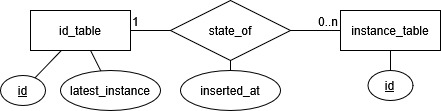
\includegraphics[scale=.6]{dateien/identity_instance_er.jpg}
\caption{Die Identität und Zustände eines Objektes in Form eines ER-Diagramms}
\label{fig:meine-grafik}
\end{figure}
Im Extraktor ist die Implementierung dieses Konzepts nur den jeweiligen Klassen bekannt, welche auf unsere Zieldatenbank zugreifen und diese manipulieren. Durch die Kapselung in den Repository-Klassen bleibt diese Implementierung den Klassen, die fachliche Funtktionen erfüllen verborgen und Datenbankzugriffe können über triviale Methoden stattfinden und vereinfachen somit die Entwicklung erheblich und reduzieren die Fehleranfälligkeit des Codes.
Dass die Datenbank später als Grundlage für einen Chatbot verwendet werden kann, beeinflusst die Art und Weise, wie Objekte in der Graphdatenbank versioniert werden. Ein Vorteil dieses Ansatzes liegt in der unkomplizierten Umsetzung. Es entfällt die Notwendigkeit, Änderungen an einzelnen Feldern zu erkennen und zu versionieren. Außerdem lässt sich der Zustand eines Objektes zu einem Zeitpunkt ohne übermäßigen Aufwand durch eine triviale Datenbankabfrage bestimmten.
Wird in einem zukünftigen Extraktionsvorgang das gleiche Objekt mit einer Änderung seiner Felder erkannt, so wird das Objekt nicht erneut angelegt, sondern lediglich als eine weitere Version dieses Objektes behandelt und in die Tabelle der Instanzen eingefügt.
\subsection{Duplikaterkennung}
Inkonsistenzen können in unserem System entstehen, wenn ein Jira-Ticket fehlerhafte Daten enthält. Existieren zwei Tickets, welche denselben Sachverhalt beschreibt handelt es sich um ein Duplikat. Beschreiben zwei Tickets den gleichen Sachverhalt sind diese nicht als Duplikat zu werten sondern weisen darauf hin, dass ein Problem möglicherweise öfters auftritt und somit schwerwiegender sein könnte. Wahre Duplikate können zu einem Ticket zusammengeführt werden. Zwei Tickets, die mit einer gewissen Wahrscheinlichkeit den gleichen Sachverhalt beschreiben können entweder bei der Übernehme in das Data Warehouse mit einem Ähnlichkeitswert versehen werden oder ohne Ähnlichkeitswert übernommen werden. Im zweiten Fall werden ähnliche oder gleiche Sachverhalten später durch den Chatbot bei Anfragen erkannt. In dieser Arbeit soll die Bestimmung eines Ähnlichkeitswertes bei der Extraktion von Daten aus dem Quellsystem geschehen. Diese Bestimmung kann mittels Künstlicher Intelligenz erfolgen oder durch eigene Applikationslogik implementiert werden. Zum anderen muss beim Design der Ähnlichkeitserkennung die Versionierung betrachtet werden. Um die Komplexität im Hinblick auf die Versionierung zu reduzieren, wird die Ähnlichkeit nur zwischen den Objekten und nicht zwischen den Versionen der Objekte berechnet. In folge dessen wird eine erneute Berechnung der Ähnlichkeiten zu anderen Tickets fällig wenn eine neue Version eines Tickets eingefügt wird. Jede dieser Berechnungen ist aufwändig und es muss ein Konzept entworfen werden um diese Berechnungen effizient durchzuführen. Eine Möglichkeit besteht darin, die Ähnlichkeitswerte nur dann erneut zu brechnen, wenn die neue Version eines Tickets signifikant von der vorherigen Version abweicht. Dazu wird das Ticket mit sich selbst verglichen.\\
Hierbei gibt es verschiedene Herausforderungen zu berücksichtigen. Zum einen muss die Rechenkomplexität beachtet werden, die sich durch das vergleichen von zwei Tickets bei allen Tickets ergibt. Die Rechenkomplexität bezeichnet den Resourcen- und Zeitbedarf einer Rechenoperation mit einer zunehmenden Anzahl n von Objekten. Dieser kann konstant, linear, quadratisch oder exponentiell sein. Im Falle des Vergleichens von Tickets steigt die Rechenkomplexität mit der Anzahl der Tickets quadratisch an [Zitat].\\
Haben sich Informationen im Quellsystem seit der letzten Übernahme geändert, so wird eine neue Version des Tickets angelegt. Eine Änderung lässt sich durch das Feld \glqq Updated\grqq\:bestimmen. Dabei handelt es sich um einen Zeitstempel der letzten Änderung. Welches Feld sich genau geändert hat ist nur durch einen aufwändigeren Abgleich mit der vorherigen Version des Tickets bestimmbar.
\subsection{Resilienz und Fehlertoleranz der Anwendung}
Heuzutage sind nahezu alle Anwendungen auf verschiedene Rechner verteilt und durch Netzwerke miteinander verbunden. Dennoch bleibt die Notwendigkeit bestehen, dass ein verteiltes System sich unverändert zu einem monolithischen System verhält. Jedoch bringen verteilte Systeme Herausforderungen mit sich, welche Maßnahmen im Design erfordern um diese Anforderung erfüllen zu können. Ein zentrales Problem bei verteilten Systemen ist die Netzwerkübertragung und die damit verbundenen möglichen Verzögerungen und Ausfällen. (vgl. van Steen, Pierre und Voulgaris (2012), S. 59-60)
\section{Implementierung und Testen}
\subsection{Implementierung der Extraktor-Komponente}
\subsubsection{Extraktion der Daten}
Die Extraktion beginnt bei Ausführung der Anwendung. Dafür muss eine Methode im Quarkus Framework konfiguriert werden. Die folgende Klasse dient mit der Methode mit der Singatur \glqq public void run()\grqq\: den Einstiegspunkt unserer Anwendung. Um eine Methode bei Initialisierung einer Java Bean zu Ausführung zu bringen muss diese mit der Annotation \glqq PostConstruct\grqq\: versehen werden. Des weiteren muss diese Methode Teil einer Klasse sein, welche als Java Bean definiert ist und somit die Annotation \glqq ApplicationScoped\grqq\: besitzt. Die Annotation \glqq Startup\grqq\: bestimmt, dass die Java Bean beim Start der Anwendung sofort initialisert wird und nicht wartet, bis diese von einer anderen Klasse verwendet wird: [ZITAT]
\begin{minted}{java}
    @Startup
    @ApplicationScoped
    public class Extraktor {
        @PostConstruct
        public void run() {
            // Run code on startup here
        }
    }
\end{minted}
Der Extraktor soll kaskadenartig vorgehen. In einem Jira-Projekt stehen viele Objekttypen mit einer 1:n Kardinalität in Verbindung (z.B Projekt und Issue oder Issue und Kommentar). Der Extraktor beginnt mit dem höchsten Objekt in der Hierarchie also einem Jira Projekt und arbeitet sich schrittweise durch alle Objekttypen. Zunächst werden für ein Jira Projekt alle relevanten Vorgänge ermittelt und extrahiert. Diese Vorgänge wiederum stehen in Beziehung mit weiteren Objekttypen, welche anschließend ebenfalls extrahiert werden. Dabei sind Felder, Kommentare, Anhänge oder die Historie des Vorgangs relevant. Außerdem soll zu jedem Vorgang auch der Vorgangstyp extrahiert werden, welcher meist die Art des Vorgangs beschreibt. Ein Vorgangstyp Bug beispielsweise verdeutlicht, dass dieser Vorgang existiert, um ein bestehendes Problem zu lösen. [ZITAT].\\
Zu Beginn des Extraktionsprozesses wird die bereitgestellte Konfiguration eingelesen. Wir benutzen hierfür die Guava Library von Google. Der Pfad, an welchem sich die Datei befindet wird mittels der Annotation \glqq ConfigProperty\grqq\: als Attribut unserer Klasse eingebracht.
\begin{minted}{java}
    @ConfigProperty(name = "extractor.config.location")
    String pathToConfig;
    
    @PostConstruct
    public void run() {
        String config = File.asCharSource(new File(pathToConfig), 
            StandardCharsets.UTF_8).read();
        for(Map<String, List<String>> project : config) {
            // Extraction process for a Jira Project goes here.
        }
    }
\end{minted}
Bei Beginn der Extraktion muss zuerst der Zeitraum bestimmt werden, für welche die Änderungen extrahiert werden. Der Beginn dieses Zeitraums entspricht dem Zeitstempel der zuletzt durchgeführten Extraktion. Der Zeitraum der letzten Extraktion kann aus der Metadaten-Datenbank ermittelt werden. Existiert noch keine Extraktion aus der Vergangenheit, so soll der Startzeitpunkt der Unix-Time herangezogen werden. Dieser entspricht dem 1. Januar 1970 um 0:00 Uhr [ZITAT]. Demnach führen wir in diesem Fall eine vollständige Extraktion der Daten durch. Hierfür nutzen wir eine eigens erstellte Klasse, welche eine Periode, im Gegensatz zur Klasse java.time.Period, durch das Speichern von zwei Zeitstempel implementiert. Wie folgt wird eine neue Periode ermittelt:
\begin{minted}{java}
    public void getPeriod() {
        Optional<Period> period = periodRepository.findLatest();
        ZonedDateTime now = ZonedDateTime.now(ZoneId.UTC);
        if(period.isPresent()) {
            return new Period(period.get().from(), now);
        } else {
            return new Period(, now);
        }
    }
\end{minted}
Für jeden Objekttyp des Jira System soll eine Extraktorklasse implementiert werden. Dazu werden fünf Klassen (Projekt, Issuetype, Issue, Subtask, Comment) benötigt. Die in den Klassen definierten Methoden zur Extraktion der Objekte werden kaskadenartig aufgerufen ähnlich zum Muster eines Baumes.\\
Die Methoden zur Extraktion, Transformation und Laden der Objekte sollen möglichst robust und fehlertolerant implementiert werden, um Ausnahmen im Extraktionsprozess behandeln zu können. Ein Ansatz zur besteht darin, Methoden erneut aufzurufen, falls eine Ausnahme bei ihrer Ausführung auftritt. Hierfür bietet das Quarkus Framework bereits die Annoation \glqq @Retry\grqq\:, welche uns ermöglicht, dieses Konzept auf eine Methode anzuwenden. Wir annotieren jede Methode die Für die Extraktion eines Objektes zuständig ist wie folgt. Unsere Methode wird vier mal erneut aufgerufen, falls eine Ausnahme auftritt:
\begin{minted}{java}
    @Retry(4)
    public void extract(Project project) {
        // Extract project here
    }
\end{minted}
Projekte besitzen, im Gegensatz zu Tickets keine Update und Create Felder, welche es ermöglichen, Änderungen im Quellsystem zu erkennen und die geänderten Projekte gezielt zu extrahieren. Daher ist eine aufwändigere Delta-Erkennung notwendig, welche für jedes konfigurierte Projekt durchgeführt werden muss. Dabei wird bei jeder Extraktion der Name, die Beschreibung und der Schlüssel gegen das bereits in der Zieldatenbank befindliche Projekt verglichen. Ergibt diese Abgleich eine Änderung, so wird eine neue Version des Projektes in die Zieldatenbank geladen. Andernfalls erfolgt keine Aktion. In jedem Fall wird danach die Extraktion der Vorgänge durchgeführt.
\subsubsection{Laden der Daten}
Ein zentrales Problem beim Laden der Daten in unser Zielsystem ist die Erkennung von bereits zuvor extrahierten und geladenen Objekten. Um ein breits in das Zielsystem geladenes Objekt zu identifizieren, kann zunächst ein eindeutiger Schlüssel festgelegt werden. Stimmt dieser Schlüssel mit einem Objekt im Zielsystem überein, wurde dieses Objekt bereits geladen und ein Match wurde gefunden. Außerdem können jedoch Sachverhalte auftreten in welchen ein Schlüssel nicht ausreichend ist, um einen Sachverhalt mittels dem Vergleich einer Zeichenkette zwei Objekte als dasselbe zu identifizieren. In folge dessen ist ein ausführlicher Vergleich verschiedener Attribute der Objekte notwendig. Sind umfangreiche Freitextfelder wie z.B Beschreibungen vorhanden, können diese mittels Künstlicher Intelligenz verglichen werden, um möglicherweise einen Match zu erkennen. Bei einem Jira-Ticket sind können verschiedene Felder, wie z.B der Titel oder die Beschreibung eines Tickets für einen Vergleich herangezogen werden.
\subsubsection{Ähnlichkeitserkennung}
Wie bereits erwähnt sollen Mechanismen implementiert werden, die Erkennung ermöglichen, ob zwei Tickets den selben oder einen ähnlichen Sachverhalt beschreiben. Um die Ähnlichkeit zweier Tickets bestimmen zu können werden die Attribute Titel und Beschreibung verwendet. Um die Ähnlichkeitsbestimmung durchzuführen wird eine neue Klasse \glqq TicketComparator\grqq\: mit der statischen Methode \glqq public static double compare(Ticket ticket1, Ticket ticket2)\grqq\: angelegt. Der Rückgabewert der Methode ist eine Gleitkommazahl zwischen den Werten 0.0 und 1.0 und beschreibt, wie ähnlich sich zwei Tickets sind. Ein Wert von 0 legt fest, dass die Tickets keine Gemeinsamkeit aufweisen. Ein Wert von 1 sagt aus, dass die beiden Tickets als exakt identisch erkannt werden:
\begin{minted}{java}
    public double compare(Ticket ticket1, Ticket ticket2) {
        final double titleSimilarity = compare(ticket1.getTitle(), ticket2.getTitle());
        final double descriptionSimilarity = compare(ticket1.getDescription(), 
            ticket2.getDescription());
        return titleSimilarity * 0.3 + descriptionSimilarity * 0.7;
    }
\end{minted}
%Welche Probleme treten bei der Ähnlichkeitserkennung auf?
% - Wann wird diese durchgeführt? Wie verhält sich das mit der Versionierung?
% - weitere recherche
\subsubsection{Quellsystem}
\subsubsection{Zielsystem}
\subsection{}
\section{Validierung und Prüfung}
\section{Fazit und Ausblick}
\section{Anhang}
\newpage
\include{literaturverzeichnis}
\section*{Eidesstattliche Erklärung}
Hiermit erkläre ich, dass ich die vorliegende Arbeit eigenständig und ohne fremde Hilfe angefertigt habe. Textpassagen, die wörtlich oder dem Sinn nach auf Publikationen oder Vorträgen anderer Autoren beruhen, sind als solche kenntlich gemacht. Die Arbeit wurde bisher keiner anderen Prüfungsbehörde vorgelegt und auch noch nicht veröffentlicht.\\\\
Ingolstadt, 18.02.2025\\\\

\includegraphics[scale=0.6]{dateien/unterschrift.png}\\
Andreas Dinauer
\end{document}

% Validierung wie?